\section{7日目}
\begin{frame}[fragile]
\frametitle{クラス}
\begin{columns}
	\column[t]{.5\hsize}
	\begin{lstlisting}[numbers=none,language=MoonScript]
class Cls
	new: (...) =>
		for i in *{...}
			table.insert @, i
	__add: (l, r) ->
		#l + #r
	__sub: (l, r) ->
		#l - #r

i1 = Cls 1, 2, 3, 4, 5
i2 = Cls 6, 7, 8

print i1 - i2 -- 2
	\end{lstlisting}
	\column[t]{.5\hsize}
	\begin{itemize}
		\item 内部的にはテーブルにメタテーブルを突っ込む感じになる。
		\item \lstinline|new|メソッドがコンストラクタになる。
	\end{itemize}
\end{columns}
\end{frame}
\section{8日目}
\begin{frame}[fragile]
	\frametitle{\lstinline|with|構文}
	\begin{columns}
		\footnotesize
		\column[t]{.49\hsize}
		\begin{lstlisting}[numbers=none,language=MoonScript]
foo = (t) ->
	i = {}

	if type(t) == "table"
		for p in *t
			table.insert i, p
	else
		setmetatable i, {t}
	
	i -- return value
		\end{lstlisting}
		\pause
		\column[t]{.01\hsize}
		\vfill
		\structure{\normalsize{}$\Rightarrow$}
		\column[t]{.49\hsize}
		\begin{lstlisting}[numbers=none,language=MoonScript]
foo_with = (t) ->
	with i = {}
		if type(t) == "table"
			for p in *t
				table.insert i, p
		else
			setmetatable i, {t}
		\end{lstlisting}
	\end{columns}
	\vspace{2\zw}

	チャンク中に変数名をバインドし、そのチャンクの戻り値とする。
\end{frame}
\section{9日目}
\begin{frame}[fragile]
	\frametitle{{\rm{}Lua\LaTeX{}}でもMoonScript}
	\begin{columns}
		\column[t]{.4\hsize}
		\tiny
		\begin{lstlisting}[numbers=none=LaTeX]
...
\usepackage{luacode}
\directlua{
	require 'lualoader'
	ms = require'moonscript.base'

	function directmoon(str)
		return (ms.loadstring(str))()
	end
}
...
\begin{luacode*}
-- オフサイドルールに気をつける
local ok, cont = pcall(directmoon,[[
for i = 1, 10
	tex.print i

tex.print "coinsLT #11"\match"(%S+)"
]])

if ok then
	tex.print("\\\\イェ〜イ")
else
	tex.print("error: ", cont)
end
\end{luacode*}
		\end{lstlisting}
		\column[t]{.6\hsize}

\alert{実行結果:}

\begin{luacode*}
local ok, cont = pcall(directmoon, [[
for i = 1, 10
	tex.print i

tex.print "coinsLT #11"\match"(%S+)"
]])

if ok then
	tex.print("\\\\イェ〜イ")
else
	tex.print("error: ", cont)
end
\end{luacode*}

\vspace{2\zw}
	非常に雑なのでいろいろ問題はある{\scriptsize{}(\lstinline|luacode*|環境じゃないとバックスラッシュなどが使えないし、逆に\lstinline|luacode*|環境だと{\rm\LaTeX{}}コマンドが簡単には使えない、等)}。
	\end{columns}
\end{frame}
\section{10日目}
\begin{frame}[fragile]
	\frametitle{なにで書く? \textcircled{1}}
	\alert{Vimでもいいんだけど}

	オープンソースなLua IDEであるZeroBrane Studio\footnote[frame]{\url{http://studio.zerobrane.com/}}%
	にはMoonScript用プラグイン\footnote[frame]{\url{https://github.com/pkulchenko/ZeroBranePackage/blob/master/moonscript.lua/}}があり、導入することでMoonScriptもバンバン書ける。
	不安定なのでバンバン落ちる。
	\begin{columns}
		\column[t]{.5\hsize}
		\tiny
		\begin{lstlisting}[numbers=none,language={[5.3]lua}]
editor.fontname = "Monaco"
editor.fontsize = 13
acandtip.droprest = true
acandtip.nodynwords = true
acandtip.startat = 2
acandtip.startegy = 2
autocomplete = true
		\end{lstlisting}
		\column[t]{.5\hsize}
		\begin{figure}[h]
			\centering
			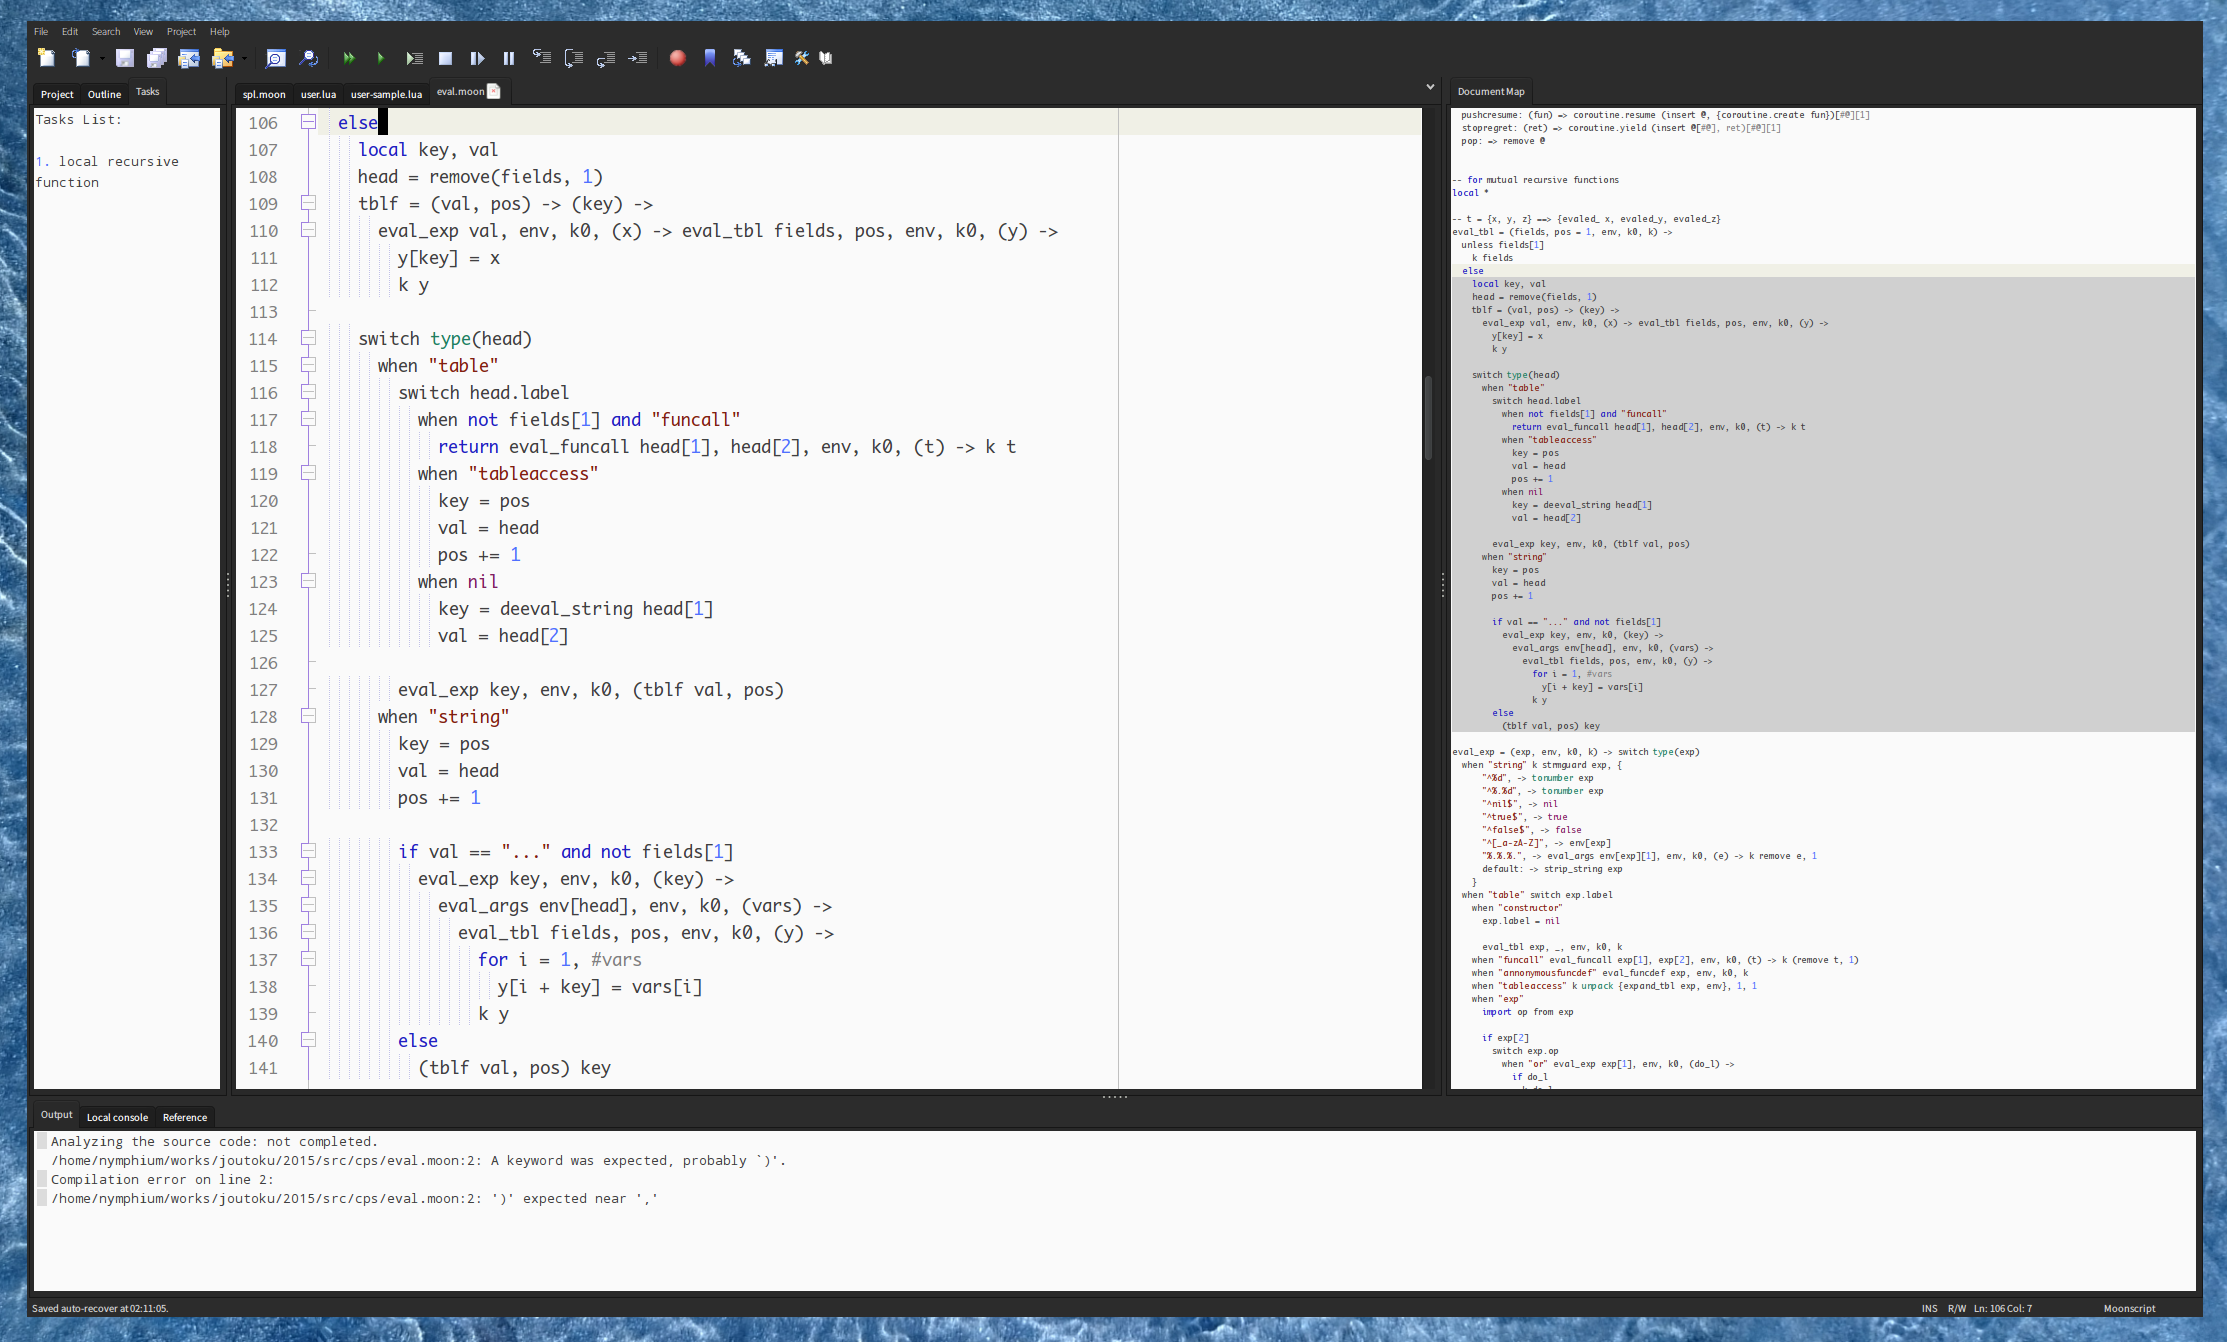
\includegraphics[width=\columnwidth]{img/zbstudio.png}
		\end{figure}
	\end{columns}
\end{frame}

\section{11日目}
\begin{frame}[fragile]
	\frametitle{なにで書く? \textcircled{2}}
	\alert{Vimでもいいんだけど}

	Howl Editor\footnote[frame]{\url{http://howl.io/}}はMoonScriptで拡張が書ける! MoonScriptも書ける! 一石二鳥!!

	\begin{columns}	
		\column[t]{.5\hsize}
		\tiny
		\begin{lstlisting}[numbers=none,language=MoonScript]
import config from howl


config.hungry_completion = true

howl.bindings.push {
	editor:
		shift_alt_c: 'editor-toggle-comment'
	ctrl_f: 'open'
	alt_e: 'cursor-word-right'
	alt_w: 'cursor-word-left'
	alt_s: 'save'
	ctrl_w:
		ctrl_w: 'quit'
	r:      'editor-redo'
	u:      'editor-undo'
}

howl.command.vi_on!
	\end{lstlisting}
	\column[t]{.5\hsize}
	\begin{figure}[h]
		\centering
		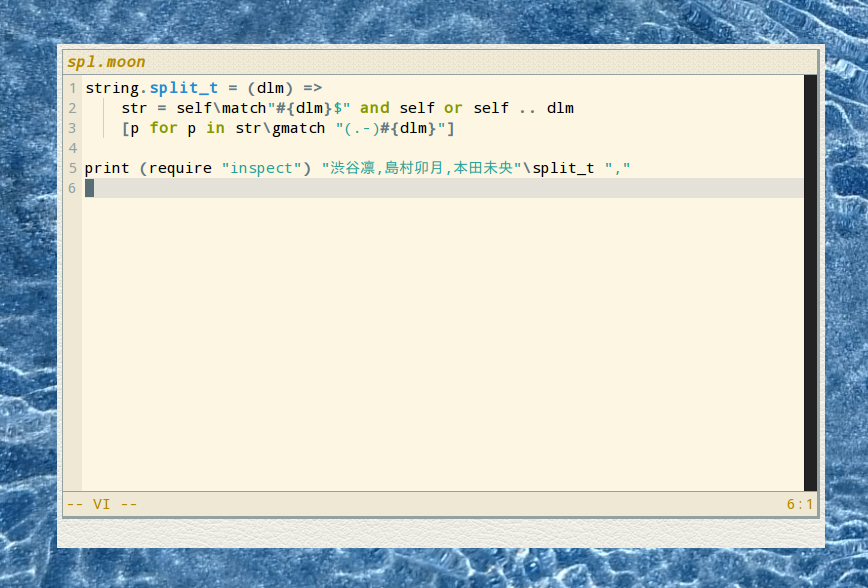
\includegraphics[width=\columnwidth]{img/howl.png}
		\end{figure}
	\end{columns}
\end{frame}
\section{12日目}
\begin{frame}[fragile]
	\frametitle{MoonScript-Luaのバージョン問題}
	MoonScriptはLua5.1ベースで開発されており\footnote[frame]{2015 12/02(commit ae2558ab67d8227b870cee1597a608c98727a924)現在}、パーサーもLua5.1までしか対応していない。

	でもLua5.3上でMoonScriptはうごくので\vspace{2\zw}

	\begin{columns}
		\scriptsize
		\newcommand{\lv}[1]{{\tiny{}(v{#1}〜)}}
		\column[t]{.5\hsize}
		\alert{これできる}
		\begin{itemize}
			\item \lstinline|__len|メタメソッド\lv{5.2}
			\item \lstinline|bit32|モジュール\lv{5.2}
			\item \lstinline|utf8|モジュール\lv{5.3}
		\end{itemize}
		\column[t]{.5\hsize}
		\alert{これできない}
		\begin{itemize}
			\item \lstinline|>>|、\lstinline|<<|演算子\lv{5.3}
			\item \lstinline|__shl|、\lstinline|__shr|メタメソッド\lv{5.3}\footnote[frame]{metatableに登録はできるが、対応する演算子が使えないため。}
			\item \lstinline;|;、\lstinline|&|演算子\lv{5.3}
			\item \lstinline|__bor|、\lstinline|__band|メタメソッド\lv{5.3}\footnotemark[10]
			\item \lstinline|//|演算子\lv{5.3}
			\item \lstinline|__idiv|メタメソッド\lv{5.3}\footnotemark[10]
			\item \lstinline|~|演算子\lv{5.3}
		\end{itemize}
	\end{columns}
\end{frame}
\begin{frame}[fragile]
	\frametitle{どうしても使いたいときは…}
	\begin{itemize}
		\begin{columns}
			\column[t]{.5\hsize}
			\item \lstinline|load|つかおう!\footnote[frame]{文字列にして\lstinline|load|につっこむため、tableそのままマズいのでサンプルでは変数名を文字列として渡している。}
				\bgroup\tiny
				\begin{lstlisting}[numbers=none,language=MoonScript]
strbin = (l, r, op) ->
	load("return #{l} #{op} #{r}")!

print(strbin(1, 10, "<<")) -- 1024

class T
	__shl: (r) =>
		table.insert @, r

t = T!
strbin "t", 3, "<<"
print(t[1]) -- 3
				\end{lstlisting}
				\egroup

			\column[t]{.5\hsize}
			\item \lstinline|require|つかおう!

				\lstinline|require|で\structure{luaファイルを}読みこめばLua処理系が処理してくれるのでOK\footnote[frame]{もちろんmoonファイルはまずMoonScriptが処理するのでパースに失敗する。}。

				\bgroup\tiny
				\begin{lstlisting}[numbers=none,language={[5.3]lua}]
-- shl.lua, callee
return 1 << 10
				\end{lstlisting}
				\begin{lstlisting}[numbers=none,language=MoonScript]
-- moon file, caller
print require 'shl' -- 1024
				\end{lstlisting}
				\egroup
		\end{columns}
	\end{itemize}
\end{frame}
